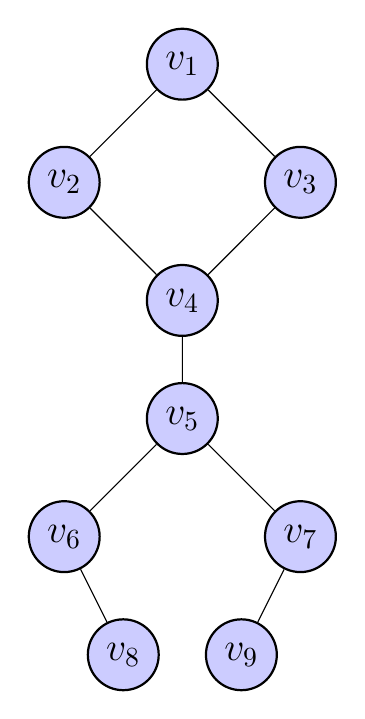
\begin{tikzpicture}[
  scale=1.5,
  vnode/.style={circle, fill=blue!20, draw=black, thick, minimum size=9mm, inner sep=0pt, font=\Large}
]
  % Vértices
  \node[vnode] (v1) at (1, 5) {$v_1$};
  \node[vnode] (v2) at (0, 4) {$v_2$};
  \node[vnode] (v3) at (2, 4) {$v_3$};
  \node[vnode] (v4) at (1, 3) {$v_4$};
  \node[vnode] (v5) at (1, 2) {$v_5$};
  \node[vnode] (v6) at (0, 1) {$v_6$};
  \node[vnode] (v7) at (2, 1) {$v_7$};
  \node[vnode] (v8) at (0.5, 0) {$v_8$};
  \node[vnode] (v9) at (1.5, 0) {$v_9$};

  % Aristas
  \foreach \from/\to in {v1/v2, v1/v3, v2/v4, v3/v4, v4/v5,
                         v5/v6, v5/v7, v6/v8, v7/v9}
    \draw (\from) -- (\to);
\end{tikzpicture}
